
\section{Calculation of active ribosomal fraction.}
\label{sec:SI_f_a}
In the main text we used the active ribosomal fraction $f_a$ that was reported
in the work of \cite{dai2016} to estimate the active ribosomal mass fraction
$\Phi_R \times f_a$ across growth conditions. We lacked any specific model to
consider how  $f_a$ should vary with growth rate, and instead find that the data
is well-approximated by fitting to an exponential curve ($f_a$ = -0.889 $e^{4.6
\cdot \lambda}$ + 0.922; dashed line in inset of \textbf{\textit{Figure 10}}(C)). We
use this function to estimate $f_a$ for each of the data points shown in
 \textbf{\textit{Figure 10}}(C).

\section{Estimation of $\langle$\#ori$\rangle$ / $\langle$\#ter$\rangle$ and $\langle$\#ori$\rangle$.}
\label{sec:SI_ori}
\textit{E. coli} shows robust scaling of cell size with the average number
of origins per cell, $\langle$\#ori$\rangle$ \citep{si2017}. Since protein makes
up a majority of the cell's dry mass, the change in cell size is also a
reflection of the changes in proteomic composition and total abundance across
growth conditions. Given the potential constraints on rRNA synthesis and changes
in ribosomal copy number with $\langle$\#ori$\rangle$, it becomes important to
also consider how protein copy numbers vary with the state of chromosomal
replication. This is particularly true  when trying to make sense of the changes
in ribosomal fraction and growth-rate dependent changes in proteomic composition
at a  mechanistic level.  As considered in the main text, it is becoming
increasingly apparent that regulation through the secondary messengers (p)ppGpp
may act to limit DNA replication and also reduce ribosomal activity in poorer
nutrient conditions.  In this context, both $\langle$\#ori$\rangle$, as well as
the $\langle$\#ori$\rangle$ / $\langle$\#ter$\rangle$ ratio become important
parameters to consider and keep track of. An increase in $\langle$\#ori$\rangle$
/ $\langle$\# ter$\rangle$ ratio  in particular, causes a relatively higher gene
dosage in rRNA and r-protein genes due to skew in genes near the origin, where
the majority of these are located

In the main text we estimated the change in $\langle$\#ori$\rangle$ with growth
rate using the nutrient-limited wild-type cell data from \cite{si2017}. We
consider their measurements of DNA replication time ($t_{C}$, 'C' period of
cell division), total cell cycle time ($t_{cyc}$, 'C' + 'D' period of cell
division), and doubling time $\tau$ from wild-type \textit{E. coli} growing
across a range of growth conditions. Here we show how we  esimate this
parameter, as well as the $\langle$\#ori$\rangle$ / $\langle$\# ter$\rangle$
ratio from their data.  We begin by considering $\langle$\#ori$\rangle$. If the
cell cycle time takes longer  than the time of cell division, the cell will need
to initiate DNA replication  more often than its rate of division, $2^{\lambda
t} = 2^{ln(2) \cdot t/ \tau}$ to maintain steady state growth. Cells will need
to do this in proportion to the ratio $\lambda_{cyc} / \lambda =  t_{cyc}/\tau$,
and the number of origins per cell (on average) is then given by $2^{t_{cyc}/
\tau}$.   The average number of termini will in contrast depend on the lag time
between  DNA replication and cell division, $t_{D}$, with
$\langle$\#ori$\rangle$ / $\langle$\# ter$\rangle$ ratio = $2^{t_{cyc}/ \tau -
t_{D}/ \tau} =  2^{t_{C}/ \tau}$.

In Figure \ref{fig:Si_tC_tcyc}(A) and (B) we plot the measured $t_{C}$ and $t_{cyc}$
values versus the doubling time from \cite{si2017}. The authors estimated
$t_{C}$ by marker frequency analysis using qPCR, while  $t_{cyc} = t_{C} +
t_{D}$ were inferred from $t_{C}$ and $\tau$. In the plots we see that both
$t_{C}$ and $t_{cyc}$ reach a minimum  at around 40 and 75 minutes,
respectively. For a C period of 40 minutes, this would correspond to a maximum
rate of elongation of about 1,000 bp/sec. Since we lacked a specific model to
describe how each of these parameters vary with growth condition, we assumed
that they were linearly dependent on the doubling time. For each parameter,
$t_{C}$ and $t_{cyc}$, we split them up into two domains corresponding to poorer
nutrient conditions and rich nutrient conditions (cut off at $\tau \approx$ 40
minutes where chromosomal replication becomes nearly constant). The fit lines
are shown as solid black lines. In Figure \ref{fig:Si_tC_tcyc}(C) and (D) we also
show $t_{C}$ and $t_{cyc}$ as a function of growth rate $\lambda$ along with our
piecewise linear fits, which match the plots in the main text.


\begin{figure}
        \centering{
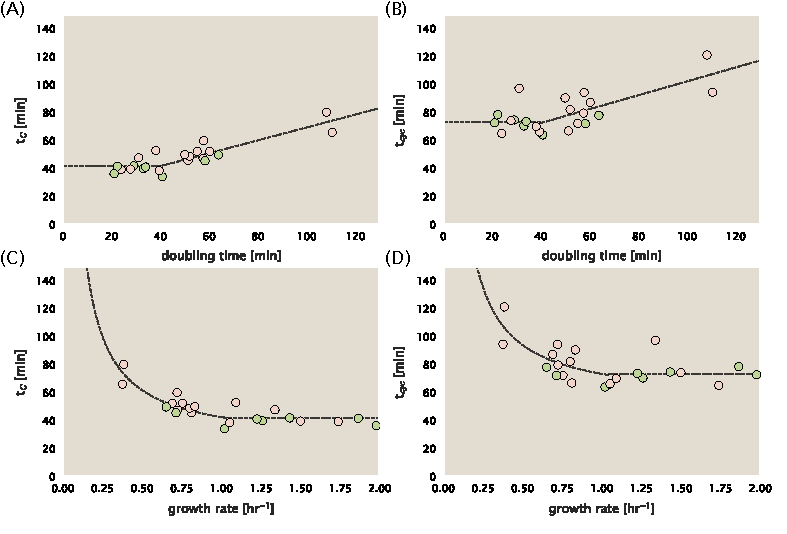
\includegraphics{SI_figs/figA10_ori_ter.pdf} \caption{\textbf{Estimation of
    $\langle$\#ori$\rangle$ / $\langle$\# ter$\rangle$ and
    $\langle$\#ori$\rangle$ using data from Si \textit{et al.} (2017).} (A) and
    (B) plot the reported $t_{C}$ and $t_{cyc}$ as a function  of cell doubling
    time $\tau$, respectively. The dashed lines show a piecewise fit to  the
    data. For short doubling times (rich media), $t_{C}$ and $t_{cyc}$ are
    assumed  constant ($t_{C}$ = 42 minutes, $t_{cyc}$ = 73 minutes). At the transition, taken to occur at 40 minutes, the
    dashed line corresponds  to an assumed proportional increase in each
    parameter as a function of the doubling time ($t_{C}$ = 0.46 $\tau$ + 23.3 minutes,
    $t_{cyc}$ = 0.50 $\tau$ + 52.7 minutes). (C) and (D) plot the same data
    as in (A) and (B), but as a function of growth rate, given by $\lambda = ln(2)/\tau$.}
\label{fig:Si_tC_tcyc} }
\end{figure}
